\ifx\wholebook\relax \else
% ------------------------

\documentclass{article}
\usepackage[en]{../../../prelude}

\setcounter{page}{1}

\begin{document}

%--------------------------

% ================================================================
%                 COVER PAGE
% ================================================================

\title{Binary Search Trees: the `hello world' data structure}

\author{Larry~LIU~Xinyu
\thanks{{\bfseries Larry LIU Xinyu } \newline
  Email: liuxinyu95@gmail.com \newline}
  }

\maketitle
\fi

\markboth{Binary search tree}{Elementary Algorithms}

\ifx\wholebook\relax
\chapter{Binary search tree, the `hello world' data structure}
\numberwithin{Exercise}{chapter}
\fi

% ================================================================
%                 Introduction
% ================================================================
\section{Introduction}
\label{introduction} \index{binary search tree}

Arrays or lists are typically considered the `hello world' data structures.
However, we'll see they are not actually particularly easy to implement. In some procedural
settings, arrays are the most elementary data structures, and it is possible to implement
linked lists using arrays (see section 10.3 in \cite{CLRS}). On the other hand, in some functional settings,
linked lists are the elementary building blocks used to create arrays and other data structures.

Considering these factors, we start with Binary Search Trees (or BST) as the `hello world'
data structure using an interesting problem Jon Bentley mentioned in `Programming Pearls'
\cite{Bentley}. The problem is to count the number of times each word occurs
in a large text. One solution in C++ is below:\index{word counter}

\lstset{language=C++}
\begin{lstlisting}
int main(int, char**) {
    map<string, int> dict;
    string s;
    while (cin >> s)
        ++dict[s];
    for(auto it = dict.begin(); it != dict.end(); ++it)
        cout << it->first << ": " << it->second << "\n";
}
\end{lstlisting}

And we can run it to produce the result using the following UNIX commands
\footnote{This is not a UNIX unique command, in Windows OS, it can be achieved
by: \texttt{type bbe.txt | wordcount.exe > wc.txt}}.

\begin{verbatim}
$ g++ wordcount.cpp -o wordcount
$ cat bbe.txt | ./wordcount > wc.txt
\end{verbatim}

The map provided in the standard template library is a kind of balanced BST
with augmented data. Here we use the words in the text as the keys and the number of
occurrences as the augmented data. This program is fast, and it reflects the power of
BSTs. We'll introduce how to implement BSTs in this section and show how
to balance them in a later section.

Before we dive into BSTs, let's first introduce the more general binary tree.

Binary trees are recursively defined. BSTs are just one
type of binary tree. A binary tree is usually defined in the following way.
\index{binary tree}

A binary tree is
\begin{itemize}
\item either an empty node;
\item or a node containing 3 parts: a value, a left child which is a binary tree and a
right child which is also a binary tree.
\end{itemize}

Figure \ref{fig:binary-tree-example} shows this concept and an example binary tree.

\begin{figure}[htbp]
  \centering
  \subcaptionbox{Concept of binary tree}{\includegraphics[scale=0.5]{img/lvr.ps}} \\
  \subcaptionbox{An example binary tree}{\includegraphics[scale=0.5]{img/btexample.ps}}
  \caption{Binary tree concept and an example.}
  \label{fig:binary-tree-example}
\end{figure}

A BST is a binary tree where the following applies to each node:
\begin{itemize}
\item all the values in left child tree are less than the value of this node;
\item the value of this node is less than any values in its right child tree.
\end{itemize}

Figure \ref{fig:bst-example} shows an example of a BST. Comparing with
Figure \ref{fig:binary-tree-example}, we can see the differences in how keys are
ordered between them.

\begin{figure}[htbp]
       \begin{center}
        \includegraphics[scale=0.5]{img/bst-1.ps}
        \caption{An example of a BST} \label{fig:bst-example}
       \end{center}
\end{figure}


% ================================================================
% Data layout
% ================================================================
\section{Data Layout}
\index{binary search tree!data layout}

Based on the recursive definition of BSTs, we can draw the
data layout in a procedural setting with pointers as in Figure
\ref{fig:node-layout-parent}.

%\begin{figure}[htbp]
%       \begin{center}
%        \includegraphics[scale=0.8]{img/node-layout.ps}
%        \caption{Node layout.} \label{fig:node-layout}
%       \end{center}
%\end{figure}

The node first contains a field for the key, which can be augmented with satellite
data. The next two fields contain pointers to the left and right children, respectively. To make backtracking to ancestors easy, a parent field is sometimes provided as well.
%Figure \ref{fig:node-layout-parent} shows the layout with parent field.

\begin{figure}[htbp]
       \begin{center}
        \includegraphics[scale=0.8]{img/node-layout-parent.ps}
        \caption{Layout of nodes with parent field.} \label{fig:node-layout-parent}
       \end{center}
\end{figure}

In this section, we'll ignore the satellite data for the sake of simplifying the illustrations. Based on this layout, the node of BST can be defined in a procedural language, such as C++:

\lstset{language=C++}
\begin{lstlisting}
template<class T>
struct node {
    node(T x):key(x), left(nullptr), right(nullptr), parent(nullptr) {}

    ~node() {
        delete left;
        delete right;
    }

    node* left;
    node* right;
    node* parent; //可选,方便succ和pred操作
    T key;
};
\end{lstlisting}

There is another setting, for instance in Scheme/Lisp languages, the elementary
data structure is a linked list. Figure \ref{fig:lisp-layout} shows how a BST node can be built on top of linked list.

\begin{figure}[htbp]
       \begin{center}
        \includegraphics[scale=0.8]{img/lisp-layout.ps}
        \caption{Binary search tree node layout on top of linked list. Where `left...' and `right ...' are either empty or BST nodes composed in the same way.} \label{fig:lisp-layout}
       \end{center}
\end{figure}

In more functional settings, it's hard to use pointers for backtracking (and typically, there is no need for backtracking, since there are usually top-down recursive solutions), and so the `parent' field has been omitted in that layout.

To simplify things, we'll skip the detailed layouts in the future and only
focus on the logic layouts of data structures. For example, below is the definition
of a BST node in Haskell:

\lstset{language=Haskell}
\begin{lstlisting}
data Tree a = Empty
            | Node (Tree a) a (Tree a)
\end{lstlisting}

% ================================================================
% Insert
% ================================================================
\section{Insertion}
\index{binary search tree!insertion}

To insert a key $k$ (sometimes along with a value in practice) to a BST $T$, we can use the following algorithm:

\begin{itemize}
\item If the tree is empty, construct a leaf node with key = $k$;
\item If $k$ is less than the key of root node, insert it in the left child;
\item If $k$ is greater than the key of root node, insert it in the right child.
\end{itemize}

The exception to the above is when $k$ is equal to the key of the root node, meaning it already exists in the BST, and we can either overwrite the data, or just do nothing. To simplify things, this case has been skipped in this section.

This algorithm is described recursively. It's simplicity is why we
consider the BST structure the `hello world' data structure. Formally,
the algorithm can be represented with a recursive mathematical function:

\be
insert(T, k) = \left \{
  \begin{array}
  {r@{\quad:\quad}l}
  node(\phi, k, \phi) & T = \phi \\
  node(insert(T_l, k), k', T_r) & k < k' \\
  node(T_l, k', insert(T_r, k)) & otherwise
  \end{array}
\right.
\ee

Where $T_l$ is the left child, $T_r$ is the right child, and $k'$ is the key when $T$ isn't empty.

The node function creates a new node given the left subtree,
a key and a right subtree as parameters. $\phi$ means NIL or empty.

Translating the above functions directly to Haskell yields the following
program:

\lstset{language=Haskell}
\begin{lstlisting}
insert Empty k = Node Empty k Empty
insert (Node l x r) k | k < x = Node (insert l k) x r
                      | otherwise = Node l x (insert r k)
\end{lstlisting}

This program utilized the pattern matching features provided by the
language. However, even in functional settings without this feature
(e.g. Scheme/Lisp) the program is still expressive:

\lstset{language=lisp}
\begin{lstlisting}
(define (insert tree x)
  (cond ((null? tree) (list '() x '()))
	((< x (key tree))
	 (make-tree (insert (left tree) x)
		    (key tree)
		    (right tree)))
	((> x (key tree))
	 (make-tree (left tree)
		    (key tree)
		    (insert (right tree) x)))))
\end{lstlisting}

This algorithm can be expressed imperatively using iteration, completely free of recursion:

\begin{algorithmic}[1]
\Function{Insert}{$T, k$}
  \State $root \gets T$
  \State $x \gets$ \Call{Create-Leaf}{$k$}
  \State $parent \gets NIL$
  \While{$T \neq NIL$}
    \State $parent \gets T$
    \If{$k <$ \Call{Key}{$T$}}
      \State $T \gets $ \Call{Left}{$T$}
    \Else
      \State $T \gets $ \Call{Right}{$T$}
    \EndIf
  \EndWhile
  \State \Call{Parent}{$x$} $\gets parent$
  \If{$parent = NIL$} \Comment{tree $T$ is empty}
    \State \Return $x$
  \ElsIf{$k <$ \Call{Key}{$parent$}}
    \State \Call{Left}{$parent$} $\gets x$
  \Else
    \State \Call{Right}{$parent$} $\gets x$
  \EndIf
  \State \Return $root$
\EndFunction
\Statex
\Function{Create-Leaf}{k}
  \State $x \gets $ \Call{Empty-Node}{}
  \State \Call{Key}{$x$} $ \gets k$
  \State \Call{Left}{$x$} $ \gets NIL$
  \State \Call{Right}{$x$} $ \gets NIL$
  \State \Call{Parent}{$x$} $ \gets NIL$
  \State \Return $x$
\EndFunction
\end{algorithmic}

While more complex than the functional algorithm, it is still fast, even when presented with very deep trees.
Complete C++ and python programs are available along with this section for reference.

\section{Traversing}
\index{binary search tree!traverse}

Traversing means visiting every element one-by-one in a BST. There are 3 ways to traverse a binary tree: a
pre-order tree walk, an in-order tree walk and a post-order tree walk. The names of these traversal methods
highlight the order in which we visit the root of a BST.

\begin{itemize}
\item pre-order traversal:, visit the key, then the left child, finally the right child;
\item in-order traversal: visit the left child, then the key, finally the right child;
\item post-order traversal: visit the left child, then the right child, finally the key.
\end{itemize}

\index{pre-order traverse} \index{in-order traverse} \index{post-order traverse}

Note that each `visiting' operation is recursive. As mentioned before, we see that the order in which
the key is visited determines the name of the traversal method.

For the BST shown in figure \ref{fig:bst-example}, below
are the three different traversal results.

\begin{itemize}
\item pre-order traversal results: 4, 3, 1, 2, 8, 7, 16, 10, 9, 14;
\item in-order traversal results: 1, 2, 3, 4, 7, 8, 9, 10, 14, 16;
\item post-order traversal results: 2, 1, 3, 7, 9, 14, 10, 16, 8, 4.
\end{itemize}

The in-order walk of a BST outputs the elements in increasing order. The definition
of a BST ensures this interesting property, while the proof of this fact is left as an exercise to the reader.

The in-order tree walk algorithm can be described as:
\begin{itemize}
\item If the tree is empty, just return;
\item traverse the left child by in-order walk, then access the key,
finally traverse the right child by in-order walk.
\end{itemize}

Translating the above description yields a generic map function:

\be
map(f, T) = \left \{
  \begin{array}
  {r@{\quad:\quad}l}
  \phi & T = \phi \\
  node(T_l', k', T_r') & otherwise
  \end{array}
\right .
\ee

Where

\[
 \begin{array}{l}
 T_l' = map(f, T_l) \\
 T_r' = map(f, T_r) \\
 k' = f(k)
 \end{array}
\]

And $T_l$, $T_r$ and $k$ are the children and key when the tree isn't empty.

If we only need access the key without create the transformed tree,
we can realize this algorithm in procedural way lie the below C++
program.

\lstset{language=C++}
\begin{lstlisting}
template<class T, class F>
void in_order_walk(node<T>* t, F f) {
    if (t) {
        in_order_walk(t->left, f);
        f(t->value);
        in_order_walk(t->right, f);
    }
}
\end{lstlisting}

The function takes a parameter f, it can be a real function, or a function
object, this program will apply f to the node by in-order tree walk.

We can simplified this algorithm one more step to define a function
which turns a BST to a sorted list by in-order traversing.

\be
toList(T) = \left \{
  \begin{array}
  {r@{\quad:\quad}l}
  \phi & T = \phi \\
  toList(T_l) \cup \{ k \} \cup toList(T_r) & otherwise
  \end{array}
\right .
\ee

Below is the Haskell program based on this definition.

\lstset{language=Haskell}
\begin{lstlisting}
toList Empty = []
toList (Node l x r) = toList l ++ [x] ++ toList r
\end{lstlisting}

This provides us a method to sort a list of elements. We can first
build a BST from the list, then output the tree
by in-order traversing. This method is called as `tree sort'.
Let's denote the list $X = \{x_1, x_2, x_3, ..., x_n\}$.

\be
  sort(X) = toList(fromList(X))
\ee

And we can write it in function composition form.

\[
  sort = toList . fromList
\]

Where function $fromList$ repeatedly insert every element to an empty
BST.

\be
  fromList(X)= foldL(insert, \phi, X)
\ee

It can also be written in partial application form\footnote{Also known as 'Curried form' to memorialize the mathematician and logician Haskell Curry.} like below.

\[
  fromList = foldL \quad insert \quad \phi
\]

For the readers who are not familiar with folding from left, this function
can also be defined recursively as the following.

\[
fromList(X) = \left \{
  \begin{array}
  {r@{\quad:\quad}l}
  \phi & X = \phi \\
  insert(fromList(\{x_2, x_3, ..., x_n\}), x_1) & otherwise
  \end{array}
\right .
\]

We'll intense use folding function as well as the function composition
and partial evaluation in the future, please refer to appendix of this
book or \cite{wiki-fold}
\cite{func-composition} and \cite{curry} for more information.

\begin{Exercise}

\begin{itemize}
\item Given the in-order traverse result and pre-order traverse result,
can you re-construct the tree from these result and figure out the
post-order traversing result?

\begin{itemize}
\item Pre-order result: 1, 2, 4, 3, 5, 6;
\item In-order result: 4, 2, 1, 5, 3, 6;
\item Post-order result: ?
\end{itemize}
\index{tree reconstruction}

\item Write a program in your favorite language to re-construct
the binary tree from pre-order result and in-order result.

\item Prove why in-order walk output the elements stored in a binary
search tree in increase order?

\item Can you analyze the performance of tree sort with big-O notation?
\end{itemize}
\end{Exercise}

% ================================================================
% Querying a binary search tree
% ================================================================
\section{Querying a binary search tree}
\index{binary search tree!search}
\index{binary search tree!looking up}

There are three types of querying for binary search tree, searching
a key in the tree, find the minimum or maximum element in the tree,
and find the predecessor or successor of an element in the tree.

\subsection{Looking up}
According to the definition of binary search tree, search
a key in a tree can be realized as the following.

\begin{itemize}
\item If the tree is empty, the searching fails;
\item If the key of the root is equal to the value to be found, the
search succeed. The root is returned as the result;
\item If the value is less than the key of the root, search in the left
child.
\item Else, which means that the value is greater than the key of the
root, search in the right child.
\end{itemize}

This algorithm can be described with a recursive function as below.

\be
lookup(T, x) = \left \{
  \begin{array}
  {r@{\quad:\quad}l}
  \phi & T = \phi \\
  T & k = x \\
  lookup(T_l, x) & x < k \\
  lookup(T_r, x) & otherwise
  \end{array}
\right .
\ee

Where $T_l$, $T_r$ and $k$ are the children and key when $T$ isn't empty.
In the real application, we may return the satellite data instead of the
node as the search result. This algorithm is simple and straightforward.
Here is a translation of Haskell program.

\lstset{language=Haskell}
\begin{lstlisting}
lookup Empty _ = Empty
lookup t@(Node l k r) x | k == x = t
                        | x < k = lookup l x
                        | otherwise = lookup r x
\end{lstlisting}

If the BST is well balanced, which means that almost
all nodes have both non-NIL left child and right child, for $n$ elements,
the search algorithm takes $O(\lg n)$ time to perform. This is not
formal definition of balance. We'll show it in later post about red-black-tree.
If the tree is poor balanced, the worst case takes $O(n)$ time to
search for a key. If we denote the height of the tree as $h$, we can
uniform the performance of the algorithm as $O(h)$.

The search algorithm can also be realized without using recursion in
a procedural manner.

\begin{algorithmic}[1]
\Function{Search}{$T, x$}
  \While{$T \neq NIL \wedge$ \Call{Key}{$T$} $ \neq x$}
    \If{$x <$ \Call{Key}{$T$}}
      \State $T \gets $ \Call{Left}{$T$}
    \Else
      \State $T \gets $ \Call{Right}{$T$}
    \EndIf
  \EndWhile
  \State \Return $T$
\EndFunction
\end{algorithmic}

Below is the C++ program based on this algorithm.

\lstset{language=C++}
\begin{lstlisting}
template<class T>
node<T>* lookup(node<T>* t, T x) {
    while (t && t->key != x) {
        if (x < t->key) t = t->left;
        else t = t->right;
    }
    return t;
}
\end{lstlisting}

\subsection{Minimum and maximum}
\index{binary search tree!min/max}

Minimum and maximum can be implemented from the property of binary search
tree, less keys are always in left child, and greater keys are in right.

For minimum, we can continue traverse the left sub tree until it is empty.
While for maximum, we traverse the right.

\be
min(T) = \left \{
  \begin{array}
  {r@{\quad:\quad}l}
  k & T_l = \phi \\
  min(T_l) & otherwise
  \end{array}
\right .
\ee

\be
max(T) = \left \{
  \begin{array}
  {r@{\quad:\quad}l}
  k & T_r = \phi \\
  max(T_r) & otherwise
  \end{array}
\right .
\ee

Both functions bound to $O(h)$ time, where $h$ is the height of the tree.
For the balanced BST, $min$/$max$ are bound to $O(\lg n)$ time,
while they are $O(n)$ in the worst cases.

We skip translating them to programs, It's also possible to implement them
in pure procedural way without using recursion.

\subsection{Successor and predecessor}
\index{binary search tree!succ/pred}

The last kind of querying is to find the successor or predecessor of an element.
It is useful when a tree is treated as a generic container and traversed with
iterator. We need access the parent of a node to make the implementation
simple.

It seems hard to find the functional solution, because there
is no pointer like field linking to the parent node\footnote{There is \texttt{ref} in ML and OCaml, but we only consider the purely functional settings.}. One solution is
to left `breadcrumbs' when we visit the tree, and use these information
to back-track or even re-construct the whole tree. Such data structure,
that contains both the tree and `breadcrumbs' is called zipper.
please refer to \cite{zipper-hbook} for details.

However, If we consider
the original purpose of providing $succ$/$pred$ function, `to traverse all the
BST elements one by one` as a generic container, we realize
that they don't make significant sense in functional settings because
we can traverse the tree in increase order by $map$ function we defined
previously.

We'll meet many problems in this series of post that they are only valid
in imperative settings, and they are not meaningful problems in functional
settings at all. One good example is how to delete an element in
red-black-tree\cite{okasaki-blog}.

In this section, we'll only present the imperative algorithm for finding
the successor and predecessor in a BST.

When finding the successor of element $x$, which is the smallest one $y$
that satisfies $y > x$, there are two cases. If the node with value $x$
has non-NIL right child, the minimum element in right child is the answer;
For example, in Figure \ref{fig:bst-succ}, in order to find the successor
of 8, we search it's right sub tree for the minimum one, which yields 9
as the result. While if node $x$ don't have right child, we need
back-track to find the closest ancestor whose left child is also ancestor
of $x$. In Figure \ref{fig:bst-succ}, since 2 don't have right sub tree,
we go back to its parent 1. However, node 1 don't have left child, so we
go back again and reach to node 3, the left child of 3, is also ancestor
of 2, thus, 3 is the successor of node 2.

\begin{figure}[htbp]
  \centering
  \includegraphics[scale=0.45]{img/bst-1.ps}
  \caption{The successor of 8, is the minimum one in its right sub tree, 9; \\
           In order to find the successor of 2, we go up to its parent 1, but 1 doesn't have left child, we go up again and find 3. Because its left child is also the ancestor of 2, 3 is the result.} \label{fig:bst-succ}
\end{figure}

Based on this description, the algorithm can be given as the following.

\begin{algorithmic}[1]
\Function{Succ}{$x$}
  \If{\Call{Right}{$x$} $\neq NIL$}
    \State \Return \textproc{Min}(\Call{Right}{$x$})
  \Else
    \State $p \gets $ \Call{Parent}{$x$}
    \While{$p \neq NIL$ and $x =$ \Call{Right}{$p$}}
      \State $x \gets p$
      \State $p \gets $ \Call{Parent}{$p$}
    \EndWhile
    \State \Return $p$
  \EndIf
\EndFunction
\end{algorithmic}

If $x$ doesn't has successor, this algorithm returns NIL.
The predecessor case is quite similar to the successor algorithm, they
are symmetrical to each other.

\begin{algorithmic}[1]
\Function{Pred}{$x$}
  \If{\Call{Left}{$x$} $\neq NIL$}
    \State \Return \textproc{Max}(\Call{Left}{$x$})
  \Else
    \State $p \gets $ \Call{Parent}{$x$}
    \While{$p \neq NIL$ and $x =$ \Call{Left}{$p$}}
      \State $x \gets p$
      \State $p \gets $ \Call{Parent}{$p$}
    \EndWhile
    \State \Return $p$
  \EndIf
\EndFunction
\end{algorithmic}

Below are the Python programs based on these algorithms. They are changed
a bit in while loop conditions.

\lstset{language=Python}
\begin{lstlisting}
def succ(x):
    if x.right is not None: return tree_min(x.right)
    p = x.parent
    while p is not None and p.left != x:
        x = p
        p = p.parent
    return p

def pred(x):
    if x.left is not None: return tree_max(x.left)
    p = x.parent
    while p is not None and p.right != x:
        x = p
        p = p.parent
    return p
\end{lstlisting}

\begin{Exercise}

\begin{itemize}
\item Can you figure out how to iterate a tree as a generic container
by using \textproc{Pred}/\textproc{Succ}? What's the performance of such traversing
process in terms of big-O?

\item A reader discussed about traversing all elements inside a
range $[a, b]$. In C++, the algorithm looks like the below code:

\texttt{for\_each (m.lower\_bound(12), m.upper\_bound(26), f);}

Can you provide the purely function solution for this problem?
\index{range traverse}
\end{itemize}

\end{Exercise}

% ================================================================
%                 Deletion
% ================================================================
\section{Deletion}
\index{binary search tree!delete}
Deletion is another `imperative only' topic for binary search tree.
This is because deletion mutate the tree, while in purely functional
settings, we don't modify the tree after building it in most
application.

However, One method of deleting element from binary search
tree in purely functional way is shown in this section. It's actually
reconstructing the tree but not modifying the tree.

Deletion is the most complex operation for binary search tree.
this is because we must keep the BST property, that for any node,
all keys in left sub tree are less than the key of this node, and
they are all less than any keys in right sub tree. Deleting a node
can break this property.

In this post, different with the algorithm described in \cite{CLRS},
A simpler one from SGI STL implementation is used.\cite{sgi-stl}

To delete a node $x$ from a tree.
\begin{itemize}
\item If $x$ has no child or only one child, splice x out;
\item Otherwise ($x$ has two children), use minimum element of its right sub tree to replace $x$, and splice the original minimum element out.
\end{itemize}

The simplicity comes from the truth that, the minimum element is stored
in a node in the right sub tree, which can't have two non-NIL children.
It ends up in the trivial case, the node can be directly splice
out from the tree.

Figure \ref{fig:del-leaf}, \ref{fig:del-1child}, and \ref{fig:del-branch}
illustrate these different cases when deleting a node from the tree.

\begin{figure}[htbp]
  \centering
  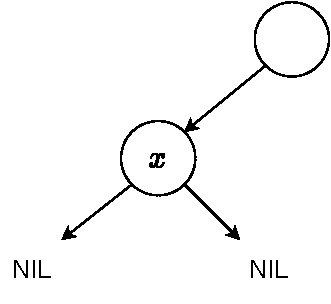
\includegraphics[scale=0.5]{img/del-leaf.ps}
  \caption{$x$ can be spliced out.} \label{fig:del-leaf}
\end{figure}

\begin{figure}[htbp]
  \centering
  \subcaptionbox{Before delete $x$.}{\includegraphics[scale=0.5]{img/del-lc-before.ps}}
  \subcaptionbox{After delete $x$, $x$ is spliced out, and replaced by its left child.}{\includegraphics[scale=0.5]{img/del-lc-after.ps}} \\
  \subcaptionbox{Before delete $x$.}{\includegraphics[scale=0.5]{img/del-rc-before.ps}}
  \subcaptionbox{After delete $x$, $x$ is spliced out, and replaced by its right child.}{\includegraphics[scale=0.5]{img/del-rc-after.ps}}
  \caption{Delete a node which has only one non-NIL child.}
  \label{fig:del-1child}
\end{figure}

\begin{figure}[htbp]
  \centering
  \subcaptionbox{Before delete $x$.}{\includegraphics[scale=0.5]{img/del-branch-before.ps}}
  \subcaptionbox{After delete $x$, $x$ is replaced by splicing the minimum element from its right child.}{ \includegraphics[scale=0.5]{img/del-branch-after.ps}}
  \caption{Delete a node which has both children.}
  \label{fig:del-branch}
\end{figure}

Based on this idea, the deletion can be defined as the below function.

\be
delete(T, x) = \left \{
  \begin{array}
  {r@{\quad:\quad}l}
  \phi & T = \phi \\
  node(delete(T_l, x), K, T_r) & x < k \\
  node(T_l, k, delete(T_r, x)) & x > k \\
  T_r & x = k \land T_l = \phi \\
  T_l & x = k \land T_r = \phi \\
  node(T_l, y, delete(T_r, y)) & otherwise
  \end{array}
\right .
\ee

Where
\[
\begin{array}{l}
T_l = left(T) \\
T_r = right(T) \\
k = key(T) \\
y = min(T_r)
\end{array}
\]

Translating the function to Haskell yields the below program.

\lstset{language=Haskell}
\begin{lstlisting}
delete Empty _ = Empty
delete (Node l k r) x | x < k = (Node (delete l x) k r)
                      | x > k = (Node l k (delete r x))
                      -- x == k
                      | isEmpty l = r
                      | isEmpty r = l
                      | otherwise = (Node l k' (delete r k'))
                          where k' = min r
\end{lstlisting}

Function \texttt{isEmpty} is to test if a tree is empty ($\phi$).
Note that the algorithm first performs search to locate the node
where the element need be deleted, after that it execute the
deletion. This algorithm takes $O(h)$ time where $h$ is the height
of the tree.

It's also possible to pass the node but not the element to the
algorithm for deletion. Thus the searching is no more needed.

The imperative algorithm is more complex because it need set the
parent properly. The function will return the root of the result tree.

\begin{algorithmic}[1]
\Function{Delete}{$T, x$}
  \State $r \gets T$
  \State $x' \gets x$ \Comment{save $x$}
  \State $p \gets $ \Call{Parent}{$x$}
  \If{\Call{Left}{$x$} $= NIL$}
    \State $x \gets $ \Call{Right}{$x$}
  \ElsIf{\Call{Right}{$x$} $= NIL$}
    \State $x \gets $ \Call{Left}{$x$}
  \Else
    \Comment{both children are non-NIL}
    \State  $y \gets $ \textproc{Min}(\Call{Right}{$x$})
    \State \Call{Key}{$x$} $\gets$ \Call{Key}{$y$}
    \State Copy other satellite data from $y$ to $x$
    \If{\Call{Parent}{$y$} $\neq x$}
      \Comment{$y$ hasn't left sub tree}
      \State \textproc{Left}(\Call{Parent}{$y$}) $\gets$ \Call{Right}{$y$}
    \Else
      \Comment{$y$ is the root of right child of $x$}
      \State \Call{Right}{$x$} $\gets$ \Call{Right}{$y$}
    \EndIf
    \If{\Call{Right}{$y$} $\neq NIL$}
      \State \textproc{Parent}(\Call{Right}{$y$}) $\gets$ \Call{Parent}{$y$}
    \EndIf
    \State Remove $y$
    \State \Return $r$
  \EndIf
  \If{$x \neq NIL$}
    \State \Call{Parent}{$x$} $\gets p$
  \EndIf
  \If{$p = NIL$}
    \Comment{We are removing the root of the tree}
    \State $r \gets x$
  \Else
    \If{\Call{Left}{$p$} $= x'$}
      \State \Call{Left}{$p$} $\gets x$
    \Else
      \State \Call{Right}{$p$} $\gets x$
    \EndIf
  \EndIf
  \State Remove $x'$
  \State \Return $r$
\EndFunction
\end{algorithmic}

Here we assume the node to be deleted is not empty (otherwise we can
simply returns the original tree). In other cases, it will first record
the root of the tree, create copy pointers to $x$, and its parent.

If either of the children is empty, the algorithm just splice $x$ out.
If it has two non-NIL children, we first located the minimum of right
child, replace the key of $x$ to $y$'s, copy the satellite data as
well, then splice $y$ out. Note that there is a special case that $y$
is the root node of $x$'s right sub tree.

Finally we need reset the stored parent if the original $x$ has only
one non-NIL child.
If the parent pointer we copied before is empty, it
means that we are deleting the root node, so we need return the new root. After
the parent is set properly, we finally remove the old $x$ from memory.

The relative Python program for deleting algorithm is given as below.
Because Python provides GC, we needn't explicitly remove the node
from the memory.

\lstset{language=Python}
\begin{lstlisting}
def tree_delete(t, x):
    if x is None:
        return t
    [root, old_x, parent] = [t, x, x.parent]
    if x.left is None:
        x = x.right
    elif x.right is None:
        x = x.left
    else:
        y = tree_min(x.right)
        x.key = y.key
        if y.parent != x:
            y.parent.left = y.right
        else:
            x.right = y.right
        if y.right is not None:
            y.right.parent = y.parent
        return root
    if x is not None:
        x.parent = parent
    if parent is None:
        root = x
    else:
        if parent.left == old_x:
            parent.left = x
        else:
            parent.right = x
    return root
\end{lstlisting}

Because the procedure seeks minimum element, it runs in $O(h)$ time on
a tree of height $h$.

\begin{Exercise}

\begin{itemize}
\item There is a symmetrical solution for deleting a node which has two
non-NIL children, to replace the element by splicing the maximum one out
off the left sub-tree. Write a program to implement this solution.
\end{itemize}

\end{Exercise}

\section{Randomly build binary search tree}
\index{binary search tree!randomly build}
It can be found that all operations given in this post bound to $O(h)$
time for a tree of height $h$. The height affects the performance
a lot. For a very unbalanced tree, $h$ tends to be $O(n)$, which leads
to the worst case. While for balanced tree, $h$ close to $O(\lg n)$.
We can gain the good performance.

How to make the binary search tree
balanced will be discussed in next post. However, there exists a simple
way. Binary search tree can be randomly built as described in \cite{CLRS}.
Randomly building can help to avoid (decrease the possibility) unbalanced
binary trees. The idea is that before building the tree, we can call a random
process, to shuffle the elements.

\begin{Exercise}

\begin{itemize}
\item Write a randomly building process for binary search tree.
\end{itemize}

\end{Exercise}

\begin{thebibliography}{99}

\bibitem{CLRS}
Thomas H. Cormen, Charles E. Leiserson, Ronald L. Rivest and Clifford Stein.
``Introduction to Algorithms, Second Edition''. ISBN:0262032937. The MIT Press. 2001

\bibitem{Bentley}
Jon Bentley. ``Programming Pearls(2nd Edition)''. Addison-Wesley Professional; 2 edition (October 7, 1999). ISBN-13: 978-0201657883

\bibitem{okasaki-blog}
Chris Okasaki. ``Ten Years of Purely Functional Data Structures''. http://okasaki.blogspot.com/2008/02/ten-years-of-purely-functional-data.html

\bibitem{sgi-stl}
SGI. ``Standard Template Library Programmer's Guide''. http://www.sgi.com/tech/stl/

\bibitem{literal-program}
http://en.literateprograms.org/Category:Binary\_search\_tree

\bibitem{wiki-fold}
http://en.wikipedia.org/wiki/Foldl

\bibitem{func-composition}
http://en.wikipedia.org/wiki/Function\_composition

\bibitem{curry}
http://en.wikipedia.org/wiki/Partial\_application

\bibitem{zipper-hbook}
Miran Lipovaca. ``Learn You a Haskell for Great Good! A Beginner's Guide''. the last chapter. No Starch Press; 1 edition April 2011, 400 pp. ISBN: 978-1-59327-283-8

\end{thebibliography}

\ifx\wholebook\relax\else
\end{document}
\fi
